\documentclass[11pt]{article}
\usepackage{geometry}                % See geometry.pdf to learn the layout options. There are lots.
\geometry{a4paper}                   % ... or a4paper or a5paper or ... 
%\geometry{landscape}                % Activate for for rotated page geometry
%\usepackage[parfill]{parskip}    % Activate to begin paragraphs with an empty line rather than an indent
\usepackage{graphicx}
\usepackage{listings}		% for listings
\usepackage{booktabs}
\usepackage{multirow}
\usepackage{amssymb}
\usepackage{epstopdf}
\DeclareGraphicsRule{.tif}{png}{.png}{`convert #1 `dirname #1`/`basename #1 .tif`.png}
\usepackage{url}

\title{Embedded system, from software to hardware\\\small{(EDAN15 VT15 Final Report)}}
\author{
Anton Eliasson, \texttt{dat11ael@student.lu.se}\\
Daniel Lundell, \texttt{ada10dlu@student.lu.se}
}
%\date{}                                           % Activate to display a given date or no date

\begin{document}
\lstset{
	language=C,
	captionpos=b,
	basicstyle=\footnotesize\ttfamily
}

\maketitle

\begin{abstract}
Brief description of the report. Context, hypothesis, experiments, results, conclusion. The abstract should contain enough
information about the rest of the document, but not too many details. Between 5--10 lines in this format.
\end{abstract}
\section{Introduction}
This is the lab report on the laboratory work in the Embedded Systems Design(EDAN15) course at LTH. The purpose of the laboratory is too use and implement an embedded system hands-on. Too see how different software and hardware solutions differ in relation to effiency, power and utilization. Starting off with pure software solution and slowly descend into hardware solutions. In addtion the purpose is to explore the framework and tool chains related to developing embedded systems. The embedded system used in the laboratory is an FPGA platform.

This part of the course is the practical part where the rest the course is more theorethical.

The rest of the report is organized as follows. Chapter 2 describe the experiments conducted throughout the 5 laboratory sessions. Chapter 3 presents the measurments and dicussions gained from the experiements in chapter 2. Chapter 4 concludes the report with a summary.


%This is the part where you give background information and prepare the reader to deal with the rest of the document. \textit{This is the final report on the laboratory work in the Embedded Systems Design (EDAN15) course, LTH \ldots} Describe the lab work organization, its relation to the rest of the course as you see it.

%\textit{The rest of the report is organized as follows. Section \ref{sec:exp} describes the experimental setup of each of the four labs. \ldots} Half a page for introduction will suffice.
\section{Experiments}\label{sec:exp}
The experiment was divided into 5 lab sessions. The goal was to evaluate software and harware solutions running on a Xilinix FPGA platform. The board used for testing was a Digilent Nexys-3. All software was developed using C.  

%mention AXI? //Daniel
%Describe overall. Xilinx ISE Design Suite 14.x Digilent Nexys-3

First laboratory was to implement and compare two pure soft-ware solution of a Greatest Common Divisor (GCD) algorithm for N numbers. Furthermore, the software has to run on a single processor system.

Second laboratory session was to implement and evaluate again a pure software solution of a gcd algorithm for N numbers. This time the architecture should use a multi-processor system. The system uses two MicroBlaze processors, working on the same data set.

Third and fourth  laboratory session was to choose a part of the gcd algorithm for N number and implement it in hardware. The hardware part was writen and simulated in VHDL using Xilinx ISE.  The hardware should input/output data following a protocol specifed in the laboratory manual.

Last laboratory session was to integrate the hardware developed in the previous session into a larger system. The system should contain software to write the necessary communication and computations, to obtain a functioning hardware/software solution for the gcd of N-numbers problem.

%Describe what you have to do as laboratory work. Describe your application, target platform. Give information about the host platform and tool chain. Use references (here and whenever appropriate elsewhere in the report) to publications \cite{microblaze} or web pages (e.g. for companies \cite{xilinx}). Do avoid giving random web pages and wikipedia as reliable sources of information.
\subsection{Software algorithms}
The software algorithm choosen was the Euclidean subtraction algorithm. This was choosen to avoid the need of calculations using division, modulo and recursion. The algorithm is very simple and well defined. 
\begin{lstlisting}[float=tbh,frame=tb,captionpos=b,caption={Euclidean subtracion algorithm},label=lst:example]
function gcd(a,b)
	while(a != b) {
		if a>b
			a = a-b
		else
			b = b-a
	}
	return a;
}
\end{lstlisting}

\subsection{Single processor}
The single processor system was implemented using a single MicroBlaze core. Software handled reading data from the serial port, calculate gcd and output it too the user. The gcd used is the one described above.
\subsection{Dual processor}
The dual processor system was implemented using two separate MicroBlaze cores. The communicated using two FSL-connections connected to each core. This was choosen over sharing memory between the two cores. Relation between the cores was divided into master/slave where one core acted as the master. The software was divided onto the two cores accordingly with the master/slave principle. Software on the master core was responsible for fetching the input data, split it and send half of it to the slave core. The slave core contained only the code for communcating through FSL and calculating gcd. Both cores calculated gcd for their half the data set. Final caluclation was done on the master core after the slave had returned the gcd for the data set on the slave core.
%Describe what is specific to this solution. How do you divide the work between the processors? How do you communicate in between them? Are there any other ways to do this? How did you make sure your solution works properly? How did you test it? Debug it in any way?
\subsection{Hardware accelerated}
The part choosen for hardware acceleration was the gcd algorithm. More specific gcd for two numbers and not N numbers. The hardware runs on a custom IP-core on the same board as the MicroBlaze core running the software. The software reads input and output each element in the data set through FSL-communication to the hardware core.  

%Describe your specific hardware accelerator. Describe the structure and behavior. Why did you choose to implement exactly this part of the algorithm? How does it fit in the whole system? How did you make sure your solution works properly? How did you test it? Debug it in any way?

Use pictures and timing diagrams, such as the one in Figure \ref{fig:example}. Do explain every picture and diagram.

\begin{figure}[!htb]
   \centering
   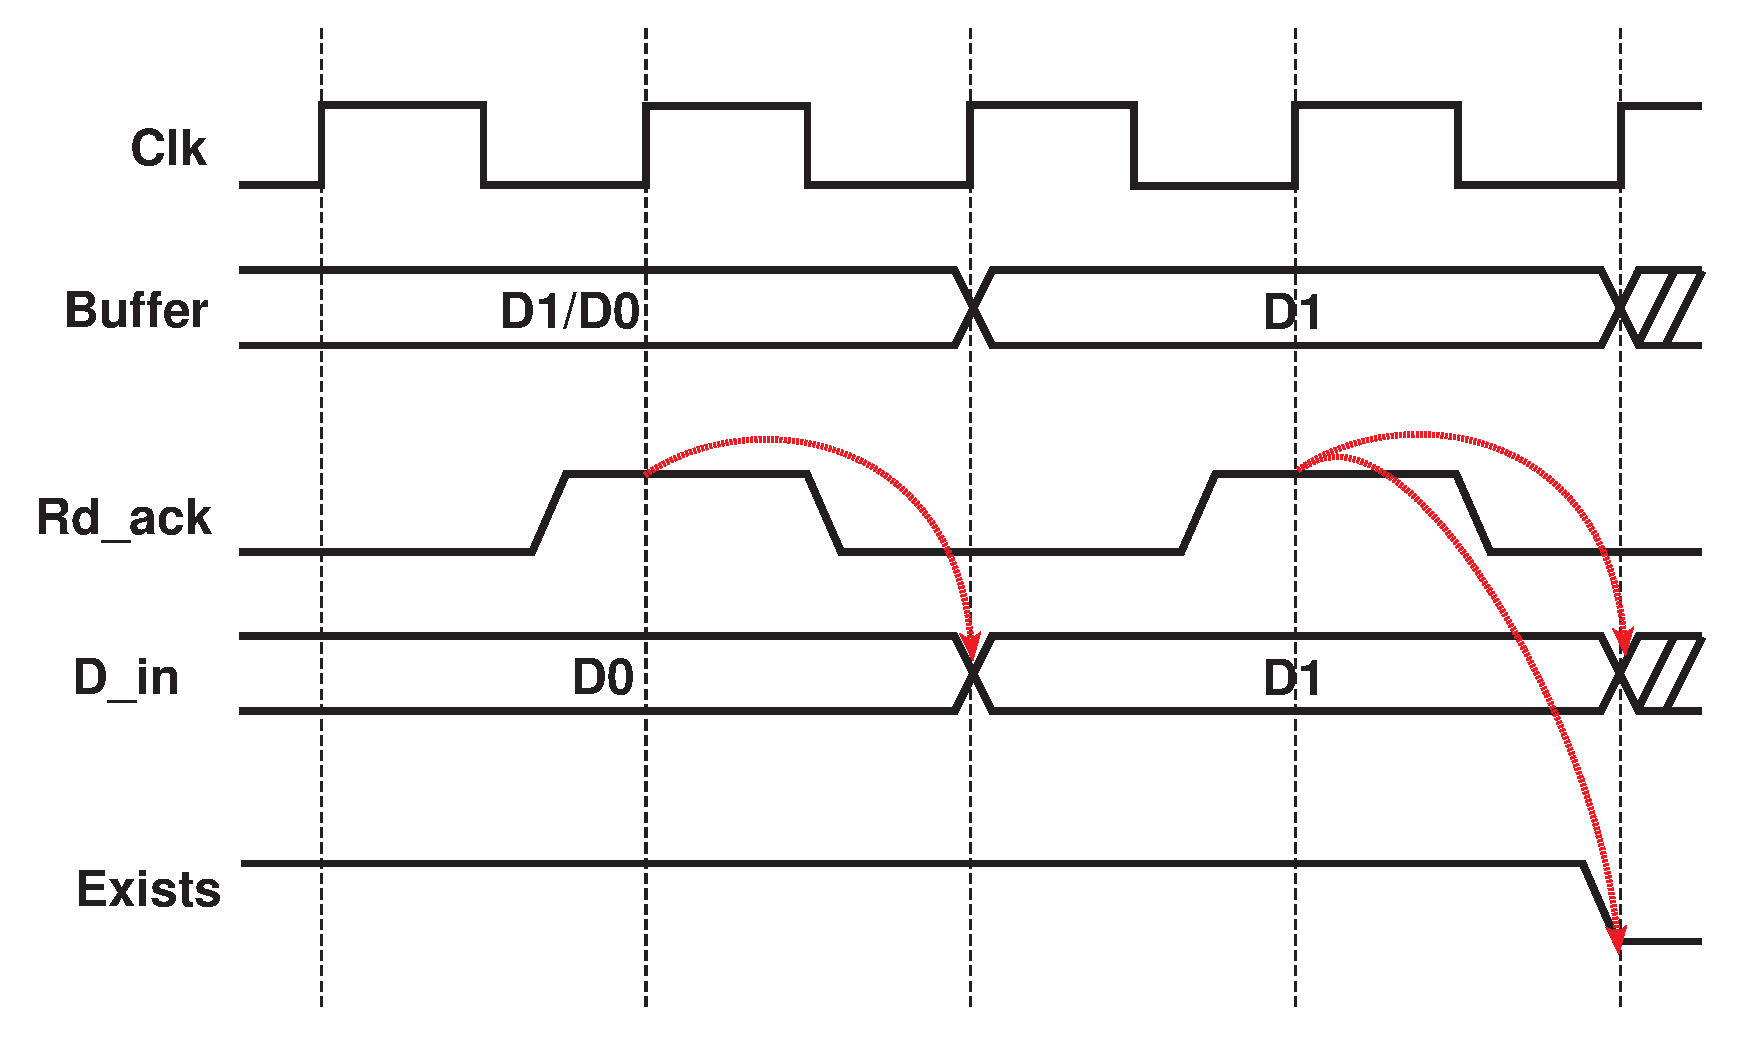
\includegraphics[width=0.6\textwidth]{example} 
   \caption{A figure example}
   \label{fig:example}
\end{figure}

\section{Measurements and Discussion}
The following chapter describes the results gained through the experiments. The clock cycles where measured when the core/cores started to share data and perform calculations. It does not include reading input or writing output through the terminal.
%This is probably the most important part of the report. In here you must describe the what and how you measure. Describe any specific parts in the hardware architecture or the software that help you conduct measurements. You should use graphs or tables to present your results, such as Table \ref{tab:example} or \ref{tab:example2}, but do not forget to describe the measures and units in the columns or graph axis.

% Requires the booktabs if the memoir class is not being used
\begin{table}[htbp]
   \centering
   %\topcaption{Table captions are better up top} % requires the topcapt package
   \begin{tabular}{@{} lcr @{}} % Column formatting, @{} suppresses leading/trailing space
      \toprule
      \cmidrule(r){1-2} % Partial rule. (r) trims the line a little bit on the right; (l) & (lr) also possible
	GCD	& Single Processor	& Dual processor	& Hardware accelerated\\
      \midrule
      10	& 24978			& 12726			&1595\\
      30	& 1992704		&  928490		&100623\\
      50	& 17097			& 9207			&2485\\
      70	& 108319		& 58745			&7688\\
     100	& 37876			&  21217		&5129\\
      \bottomrule
   \end{tabular}
   \caption{Clock cycles using the different solutions explained in chapter 2.}
   \label{tab:Clockcycles}
\end{table}

%\begin{table}[htbp]
%   \centering 
% \begin{tabular}{cc|c|c|c|c|l}
%\cline{3-6}
%& & \multicolumn{4}{|c|}{Primes} \\ \cline{3-6}
%& & 2 & 3 & 5 & 7 \\ \cline{1-6}
%\multicolumn{1}{|c|}{\multirow{2}{*}{Powers}} &
%\multicolumn{1}{|c|}{504} & 3 & 2 & 0 & 1 &     \\ \cline{2-6}
%\multicolumn{1}{|c|}{}                        &
%\multicolumn{1}{|c|}{540} & 2 & 3 & 1 & 0 &     \\ \cline{1-6}
%\multicolumn{1}{|c|}{\multirow{2}{*}{Powers}} &
%\multicolumn{1}{|c|}{gcd} & 2 & 2 & 0 & 0 & min \\ \cline{2-6}
%\multicolumn{1}{|c|}{}                        &
%\multicolumn{1}{|c|}{lcm} & 3 & 3 & 1 & 1 & max \\ \cline{1-6}
%\end{tabular}
%  \caption{Uses \textit{multirow} \LaTeX package}
%   \label{tab:example2}
%\end{table}
Say a few words about the complexity of the different solutions and how long did it take to reach a working design.
 
\subsection{Performance}
The performance figures are presented in Listing 1. When using the single and dual processor solution only software was used together with hardware support from the board. When comparing the single and dual processor solution its quite easy to see that the required cycles are almost half of the single processor. This includes sending data through the FSL, still its almost half as fast. Its not very suprising since each core only have to calculate half the dataset in the dual processor solution. This was not quite expected, we expected the FSL link to require more clock cycles. A faster solution could probably be found using direct memory sharing between the two cores. This would reduced the need for sending data over the FSL link but it might increase some time waiting when writing to memory to avoid overwriting data.

The hardware accelerated solution is significantly faster than both the single and dual processor solution. The custom IP core written in VHDL is significantly faster than the MicroBlaze core. The gcd algorithm is moved completley to a hardware solution. The MicroBlaze core is only responsible for FSL communication(and input/output but its not measured). A drawback with our solution is the lack of a gcd for N numbers, ours only provide a gcd for 2 numbers. This requires our VHDL core to wait for the MicroBlaze core each calculation. A faster solution could bave been implemented using a N number gcd in VHDL. Our expectations where quite right, we assumed the hardware solution would be faster but not that much faster. We also assumed we wouldnt get a fast result due to the 2 number gcd instead of the N number gcd.

In Listing 1 its easy to see that the clock cycles required to calculate the gcd with 30 numbers is very much slower than the rest. This is due to a drawback in the euclidean algorithm. The effciency is described by the number of divisions required[REFERENCE:WIKI:The Art of computer programming]. Our version uses the subtraction method so instead of division requried its described by the number of subtractions needed. In the sample data(found at cs.lth.se/edan15/labs/assignments) it can be seen that the gcd for the file contaning 30 numbers is 3 while the gcd for 100 numbers is 587. It can also be noted that the number range is quite similar in both the sample files. This requires our algorithm to do a significant more amount of subtractions in the file contaning 30 numbers than the one containing 100 numbers. This increases the number of clock cycles required to calculate the gcd.


%How about compiler optimizations? 


\subsection{Device Utilization}
Give the FPGA resources consumed by each of your solutions. Explain how these relate to each other -- e.g. whether a dual processor system has double the area of a single processor system and how do these relate to the hardware accelerated solution. Explain why or how using different algorithms influences or not the device utilization.


\begin{table}[htbp]
   \centering
   %\topcaption{Table captions are better up top} % requires the topcapt package
   \begin{tabular}{@{} lcr @{}} % Column formatting, @{} suppresses leading/trailing space
      \toprule
      \cmidrule(r){1-2} % Partial rule. (r) trims the line a little bit on the right; (l) & (lr) also possible
	Name	& Single Processor	& Dual processor	& Hardware accelerated\\
      \midrule
      Number of slice registers	& 24978			& 12726			&1595\\
      Number of slice LUT	& 1992704		&  928490		&100623\\
      Number of occupied slices	& 17097			& 9207			&2485\\
      70	& 108319		& 58745			&7688\\
     100	& 37876			&  21217		&5129\\
      \bottomrule
   \end{tabular}
   \caption{Clock cycles using the different solutions explained in chapter 2.}
   \label{tab:Utilization}
\end{table}

\subsection{Power and Energy}
The power and energy consumption are also important for a design. The XPower Analyser that comes with the Xilinx ISE helps you determine the power consumption for your designs. Have a look at the hierarchical breakdown of power consumption and identify the parts of your design that consume a lot of power. Also, as you know energy is the time integral of power:
\begin{equation}
E = \int_{t_1}^{t_2} P dt \approx P \Delta t
\end{equation}
How do your different solutions compare from the power and energy consumption point of view?

\section{Summary}
It has become very clear during the sessions how software and hardware relate to each other in question of performance.
%In this part you briefly summarize your report. Continue with conclusions, lessons learned, unexpected results, unsolved problems or other issues that remain open. Relate back to the content of the course and explain whether or how the laboratory work helped you or not with understanding certain issues from the theoretical part.

\bibliographystyle{plain}
\bibliography{abibfile}

\end{document}  
